%!TEX root = ../thesis.tex

%jama -- micro-level simulation results and GA calibration chapter

\chapter{Micro-Level Simulation Results and GA Calibration}
\label{ch:micro_results}

This chapter presents the open-loop simulation results of the agent-based micro model.
In this context, \emph{open-loop} means that the model is driven by fixed or externally prescribed transmission-rate trajectories rather than by MPC feedback.
The closed-loop results - where the MPC-generated $\beta(t)$ drives the ABM --- are presented in Chapter~\ref{ch:closed_loop}.

\section{Baseline Uncontrolled Epidemic}
\label{sec:baseline_micro}

%jama
Under a constant transmission rate $\beta_1 = \beta_2 = 0.45$ with $N = 1\,000$ agents and no initial vaccination, the model produces a single epidemic wave with a clear infection peak followed by decline as the susceptible pool is depleted.
Figure~\ref{fig:population_stack} shows the evolution of all compartments over 150~days.

\begin{figure}[ht]
  \centering
  
\includegraphics[width=0.85\textwidth]{{Figures/jama/Population state stack}}
  \caption{%jama
    Population state evolution over 150~days under a constant uncontrolled transmission
    rate $\beta = 0.45$. The stacked trajectories summarise how agents move between
    epidemiological states over time.}
  \label{fig:population_stack}
\end{figure}

Because the model is stochastic, repeated runs reveal variation across realisations consistent with the binomial character of the daily transition draws.
At $\beta = 0.45$ and $\gamma = 1/12$, the basic reproduction number is $R_0 = \beta/\gamma = 5.4$, well above the epidemic threshold, producing a large initial wave consistent with compartmental ODE theory \citep{kermack1927}.

\section{Effect of the Transmission Rate}
\label{sec:beta_sweep}

%jama
A parameter sweep over constant values of $\beta$ confirms the expected monotone relationship: higher $\beta$ produces a larger and earlier peak infected count $\max_t I(t)$, providing empirical validation that the mean-field infection probability in Equation~\eqref{eq:pinf_S} drives aggregate dynamics consistent with compartmental ODE theory.
Specifically, for $\beta \in \{0.20, 0.30, 0.40, 0.45\}$, each increment in $\beta$ produces both a higher peak and an earlier peak day, confirming that the ABM reproduces the qualitative behaviour expected from SIR theory.

\section{Two-City Comparison}
\label{sec:two_city_results}

%jama
The two-city structure produces heterogeneous regional dynamics even when both cities are initialised with similar conditions.
Figure~\ref{fig:city_comparison} shows the infected and hospitalised trajectories for City~1 and City~2 under the MPC-driven $\beta(t)$ signal.

\begin{figure}[ht]
  \centering
  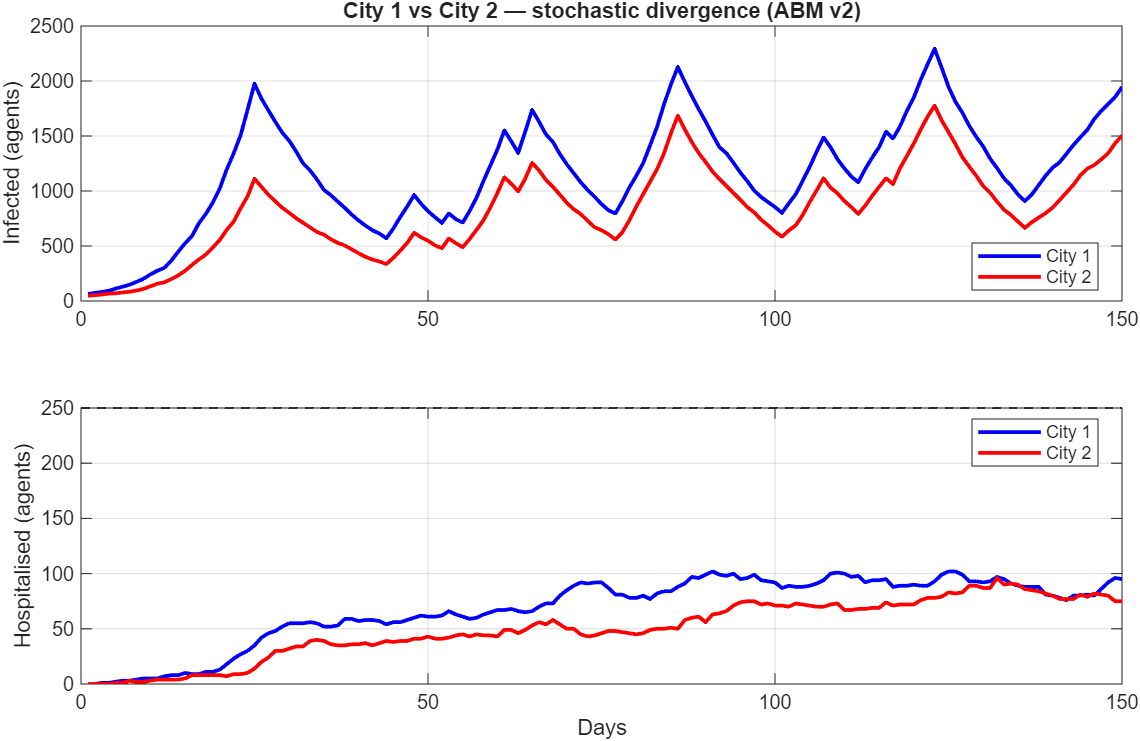
\includegraphics[width=0.85\textwidth]{Figures/jama/city_comparison_uploaded}
  \caption{%jama
    Stochastic divergence between City~1 (blue) and City~2 (red) under the
    MPC-driven transmission rate over 150~days.
    Top panel: infected agents $I(t) + I_v(t)$;
    bottom panel: hospitalised agents $H(t)$, with dashed line at per-city hospital capacity.
    City~1 consistently leads in both metrics due to amplification of initial
    stochastic differences through commuting coupling.}
  \label{fig:city_comparison}
\end{figure}

Figure~\ref{fig:per_city_hosp} shows the per-city hospital load in more detail.

\begin{figure}[ht]
  \centering
  
\includegraphics[width=0.85\textwidth]{{Figures/jama/Per-city hospital load}}
  \caption{%jama
    Per-city hospital load over 150~days under the MPC-driven transmission rate.
    Both cities remain within capacity, but City~1 sustains a persistently higher burden.}
  \label{fig:per_city_hosp}
\end{figure}

City~1 sustains a persistently higher burden, demonstrating that small stochastic seeding differences are amplified through inter-city commuting into a persistent inter-city disparity that ODE models can only represent in expectation.
This behaviour is a key feature that the micro model reveals and that the aggregate macro model cannot capture.

\section{GA Calibration}
\label{sec:ga_calib}

%jama
The macro ODE model and the agent-based model operate at different levels of abstraction.
Even when nominal parameter values are matched, their outputs may diverge because the ABM includes stochastic transmission events and individual-level interactions, whereas the macro model represents population averages through deterministic compartment dynamics.
As a result, direct analytical calibration between the two model classes is not feasible.

\subsection{Calibration Strategy}
\label{sec:ga_strategy}

%jama
To address this mismatch, a genetic algorithm (GA) is used as a derivative-free optimisation method capable of handling noisy and nonlinear objective functions.
The GA iteratively searches for parameter values that minimise the discrepancy between the macro and micro models.
Each candidate solution is a parameter vector
\begin{equation}
  \theta = (\beta_1,\; \gamma,\; h),
\end{equation}
where $\beta_1$ is the transmission parameter, $\gamma$ is the recovery rate, and $h$ is the hospitalisation rate in the macro ODE model.
For each candidate vector, the ODE model is simulated and its hospital load trajectory is compared with the mean hospital load produced by the ABM.

\subsection{Objective Function}
\label{sec:ga_objective}

%jama
The objective function is defined as the symmetric mean absolute percentage error (sMAPE) between the ODE hospital load $H_{\mathrm{ODE}}(t)$ and the average ABM hospital load $H_{\mathrm{ABM}}(t)$ over the simulation horizon:
\begin{equation}
  J(\theta) = \frac{1}{T} \sum_{t=1}^{T} \frac{|H_{\mathrm{ODE}}(t) - H_{\mathrm{ABM}}(t)|}{H_{\mathrm{ABM}}(t)}.
  \label{eq:mape}
\end{equation}
Additionally, a penalty term is included in the calibration procedure to account for mismatches in peak values, so that both the amplitude and timing of the epidemic peak are captured more faithfully.

Hospital load is selected as the calibration target because it is the primary controlled variable in the MPC formulation and directly reflects the critical healthcare-capacity constraint.
Aligning the hospital-load dynamics therefore ensures that the controller is calibrated against the variable that matters most for intervention design.

\subsection{Calibration Results}
\label{sec:ga_results}

%jama
Figure~\ref{fig:ga_calib} shows the GA calibration outcome: the fitted ODE hospital load trajectory alongside the mean ABM hospital load across seven scenario types.

\begin{figure}[ht]
  \centering
  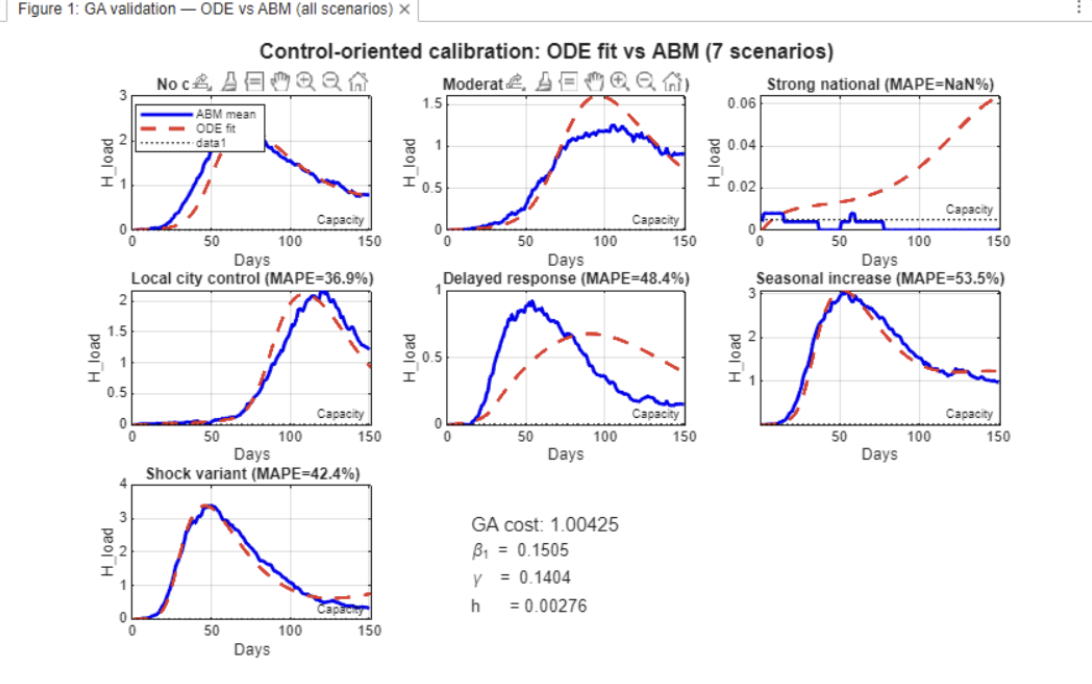
\includegraphics[width=0.90\textwidth]{Figures/jama/ga_validation_uploaded}
  \caption{%jama
    GA calibration: ODE fit (red dashed) versus ABM mean (blue solid) hospital load
    $H_{\mathrm{load}}(t)$ across seven scenario types.
    The ``Strong national'' panel reports MAPE\,=\,NaN because the ABM hospital
    load is effectively zero under aggressive suppression.
    Remaining scenarios yield MAPE of 36.9--53.5\%, reflecting inherent ABM
    stochasticity and the ODE aggregate approximation.
    Calibrated parameters: $\beta_1 = 0.1505$, $\gamma = 0.1404$, $h = 0.00276$.}
  \label{fig:ga_calib}
\end{figure}

The calibrated parameters are $\beta_1 = 0.1505$, $\gamma = 0.1404$, and $h = 0.00276$, yielding a final GA cost of 1.00425.
These values reduce the discrepancy between the macro and micro models, helping both representations operate within the same epidemiological regime.
This alignment is essential for validating that MPC decisions derived from the macro model remain meaningful when applied to the stochastic agent-based simulation.

The GA optimisation variables are constrained by:
$\beta_1 \in [0.05,\, 0.5]$,
$\gamma \in [0.05,\, 0.2]$,
$h \in [0.001,\, 0.1]$.
The fitness function minimises the hospital-load MAPE with the additional peak-alignment penalty described in Equation~\eqref{eq:mape}.

\section{Summary}
\label{sec:micro_summary}

%jama
The agent-based micro model complements the macro-level epidemic description by representing individual agents, stochastic state transitions, and city-specific dynamics.
Its main characteristics can be summarised as follows:
\begin{enumerate}
  \item It uses a seven-state compartment structure that aligns with the disease categories used at the macro level.
  \item It supports both a mean-field non-visual simulation and a spatially explicit visual simulation.
  \item It incorporates vaccination, waning immunity, hospitalisation, and fatality through stochastic daily transitions.
  \item It models a two-city setting with separate transmission inputs and, in the visual case, stochastic commuting.
  \item It provides aggregate compartment counts that can be used for comparison with or coupling to a macro-level model.
\end{enumerate}
At the same time, the present implementation remains deliberately simple.
It does not include age structure, social-contact networks, or large-scale demographics.
These omissions are acceptable for a compact thesis prototype, but they also indicate clear directions for future development (see Section~\ref{sec:future}).
